\subsection{Bayesian changepoint detection}\label{sec:results_bayesian}
%noc utili per fare riferimento ai grafici, in compenso sono poche parole
% Che significa "dinamiche strutturali"? 
%strutturali nel senso che superano il solo sport o il solo gdp ma coinvolgono 
%la struttura di tutto l'approccio di un intero stato
%e in quanto tali persistono anche in altre edizioni in cui non ospitano

%teoria incubazione c'è scritto che "denominiamo" quindi noi qui ed ora, no fonti
%se ti da fastidio si puo togliere


\subsubsection{Risultati: Casi di Conferma}
I risultati rivelano una convergenza temporale che, nei casi più emblematici,
ridefinisce le dinamiche strutturali del vantaggio olimpico. Per la Cina (CHN), il
modello identifica la svolta del PIL nel 1993 e la svolta del medagliere nel
2004: un \textit{lead effect} di undici anni. Il PIL in forte espansione ha
dunque preceduto e, con ogni probabilità, finanziato la costruzione del sistema
sportivo che ha prodotto il dominio cinese a partire dai Giochi di Atene,
raggiungendo il proprio apice a Pechino 2008. 
Analogamente, per la Gran Bretagna (GBR), il modello rileva la svolta economica nel 1999 e quella atletica nel 2008,
configurando un anticipo di nove anni compatibile con i tempi di costruzione del
programma UK Sport. Per l'Australia (AUS), il lead è più lungo. 28 anni tra la svolta
del PIL nel 1968 e quella del medagliere nel 1996, ma coerente con la
costruzione delle strutture che hanno preceduto Sydney 2000.

% questo lo sposterei dopo e unirei con la conclusione alla fine

Questi tre casi supportano quantitativamente quella che denominiamo Teoria dell' Effetto
Incubazione: la spinta del PIL fornisce la copertura finanziaria per un
investimento sistemico nello sport, il cui rendimento si materializza nel
medagliere con un ritardo variabile, che tende a consolidarsi nelle edizioni
successive all'evento casalingo.

\subsubsection{Limiti del Modello e Casi Anomali}

% cosa è "teoria del lead-lag"? https://en.wikipedia.org/wiki/Lead%E2%80%93lag_effect
% strutturale messo in molti posti non lo capisco 
%spiegato sopra. se in altra accezione su un arottura nel grafico, termine tecnico
%per non indicare una momentanea fluttuazione
%ti rispiego decoupling, si riferisce al pil che continua a crescere mentre 
%il medagliere si ferma, quindi i due trend si decouplano

Un'analisi rigorosa impone di affrontare esplicitamente i casi in cui il
modello produce risultati divergenti dalla teoria del lead-lag.

Il caso italiano (ITA) è il più istruttivo: il modello individua una svolta simultanea
di PIL e medagliere nel 1968, sulla scia dei Giochi di Roma 1960, ma nelle
decadi successive le due serie si disaccoppiano (\textit{decoupling}):
il PIL cresce in modo sostenuto fino ai primi anni 2000, mentre il medagliere
subisce una flessione strutturale e cambia rotta. Questo suggerisce che oltre
una certa soglia di sviluppo economico, la variabile discriminante non sia
la crescita del PIL, ma l'allocazione delle risorse verso nella direzione giusta.

Il Brasile (BRA) presenta un'inversione temporale: la svolta del medagliere nel 1996
precede quella del PIL nel 2007, suggerendo che in certi contesti sia
l'ambizione olimpica a innescare l'investimento, e non viceversa. Il Giappone (JPN),
con un lag di 52 anni tra le due svolte, costituisce invece un artefatto del
modello: la stazionarietà pluridecennale del medagliere e il picco isolato di
Tokyo 2020 rendono il changepoint atletico statisticamente poco affidabile, come
confermato dalla distribuzione a posteriori piatta. Gli Stati Uniti (USA), infine, con 
quattro edizioni ospitate e una dominanza ininterrotta, generano un livello di rumore 
tale da rendere qualsiasi inferenza causale non interpretabile nel framework adottato.

\begin{figure}[H]
    \centering
    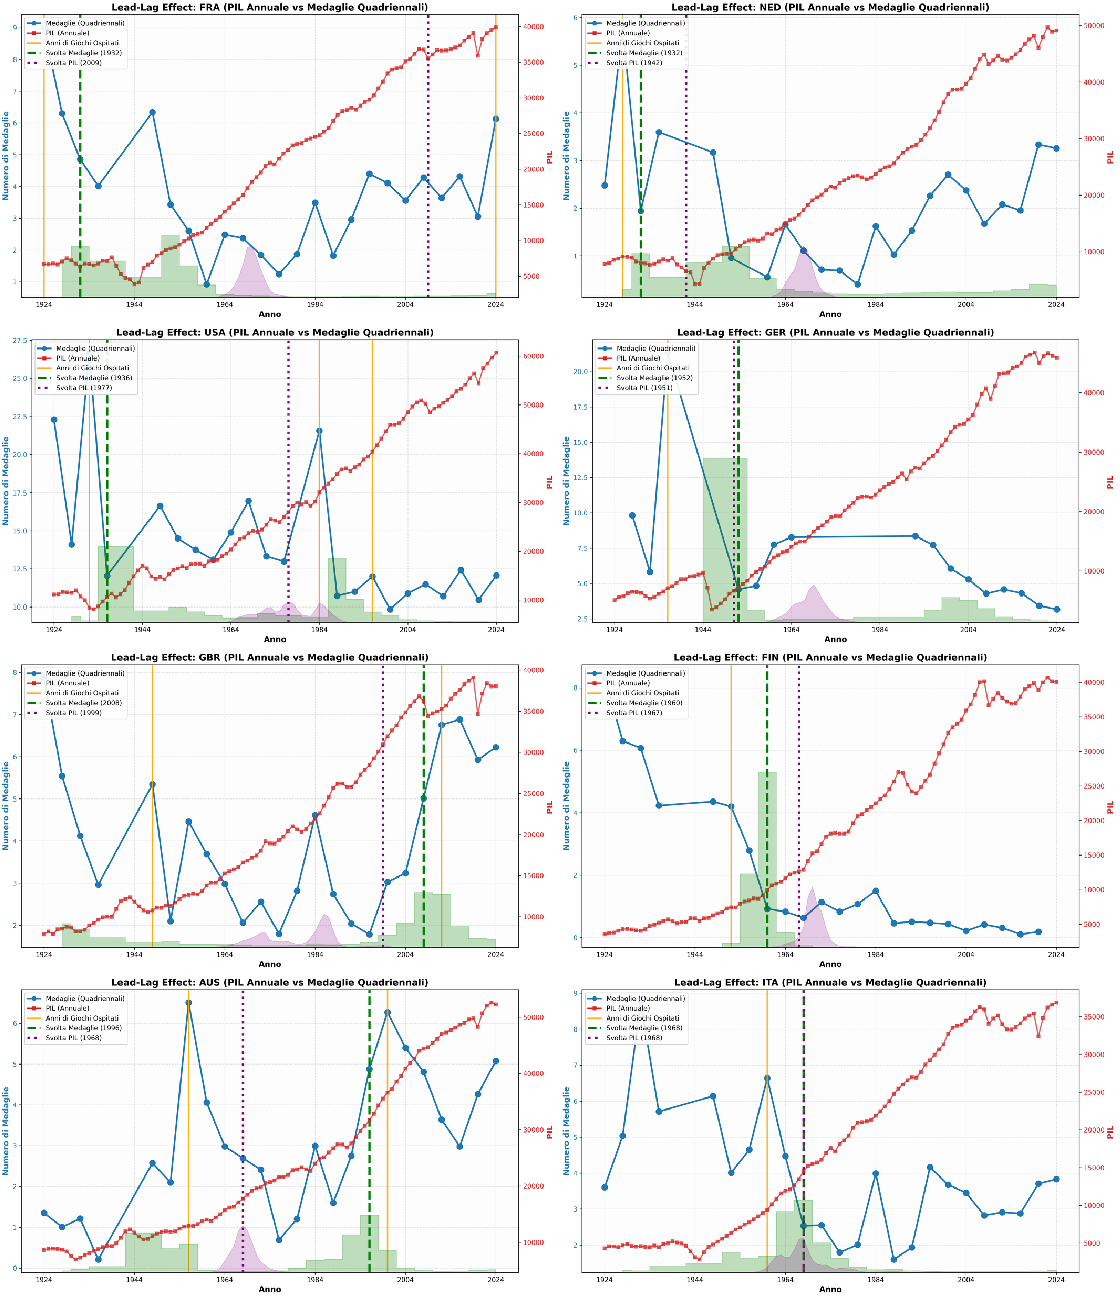
\includegraphics[width=\linewidth]{../../docs/img/Bayesian_plot1.pdf}
    \caption{Changepoint Detection per PIL e Medagliere in Nazioni
    Ospitanti(1).\\
	La distribuzione di probabilità a posteriori normalizzata è visualizzata
	come area ombreggiata. }
    \label{fig:bayesian_img1}
\end{figure}

\begin{figure}[H]
    \centering
    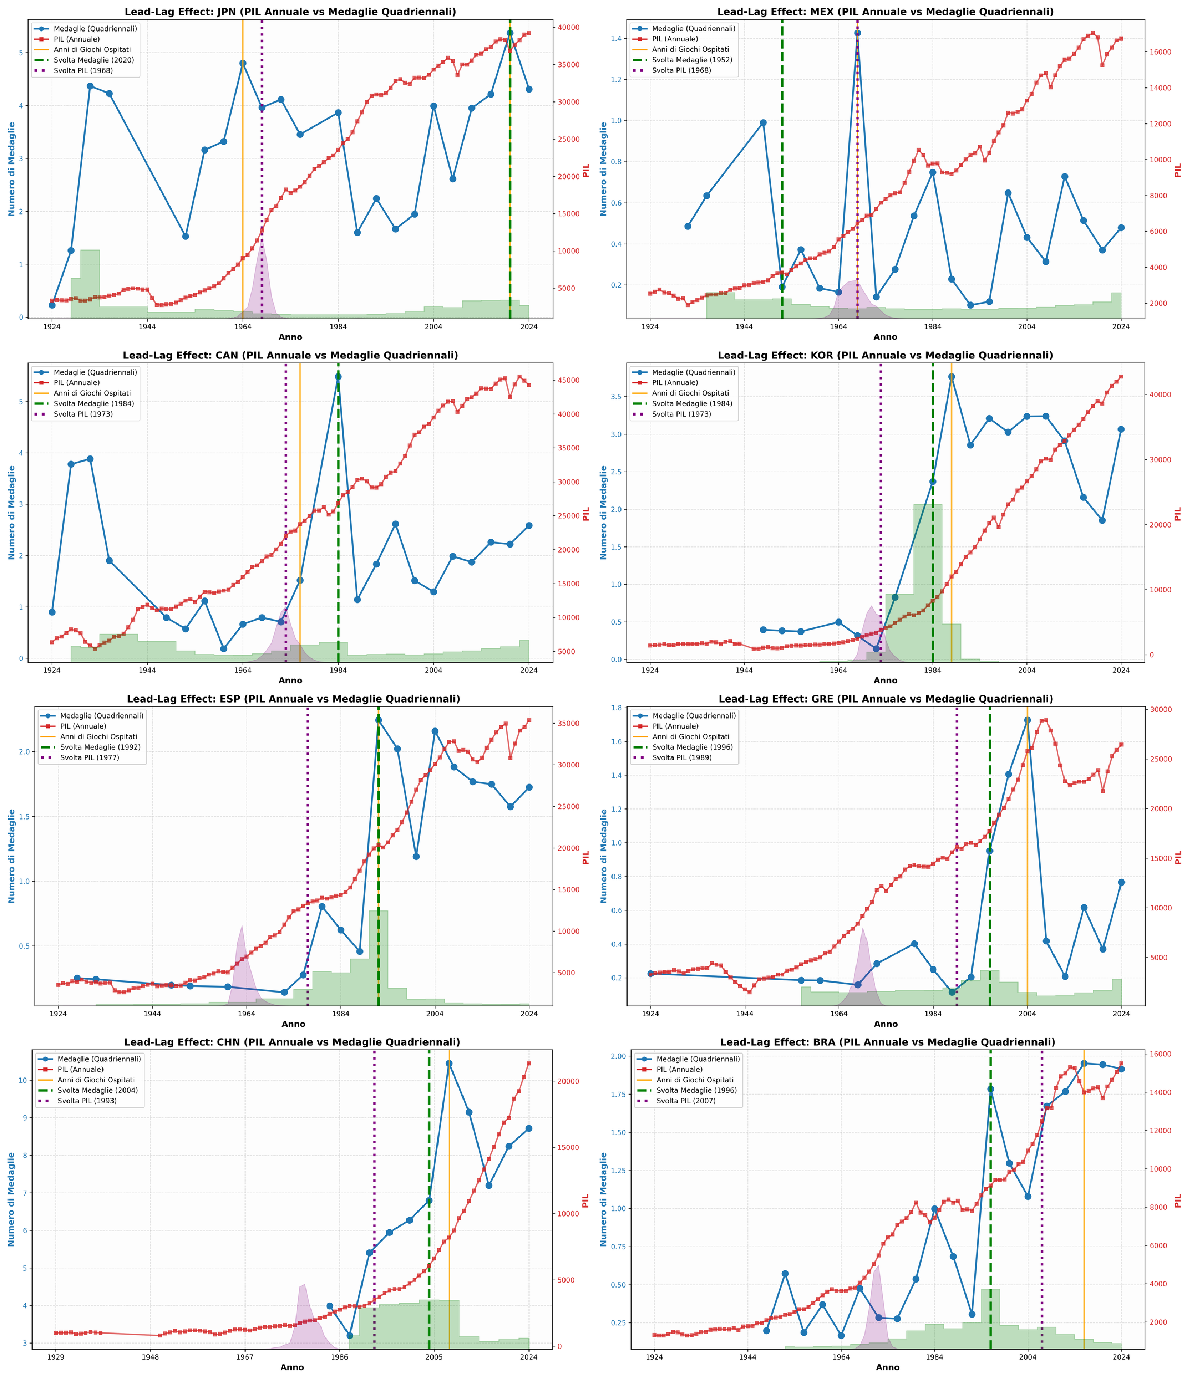
\includegraphics[width=\linewidth]{../../docs/img/Bayesian_plot2.pdf}
    \caption{Changepoint Detection per PIL e Medagliere in Nazioni
    Ospitanti(2).\\
	La distribuzione di probabilità a posteriori normalizzata è visualizzata
	come area ombreggiata.}
    \label{fig:bayesian_img2}
\end{figure}


% È un riassunto che non aggiunge informazioni (risultati) a quanto già detto.
% Ci si può fare un cenno nella conclusione (dove cercheremo di parlare di tutti
% i metodi insieme, per risparmiare spazio).

%\subsubsection{Il PIL come Architetto, non come Catalizzatore}
%
%Nei Paesi in forte espansione come Cina, Gran Bretagna, Australia, il PIL
%agisce da \textit{architetto} del successo olimpico: la sua crescita
%strutturale abilita investimenti che si manifestano nel medagliere con un
%anticipo di uno o due cicli olimpici, mentre l'assegnazione dei Giochi funge da
%catalizzatore di un processo già in corso. Dove invece le risorse esistono ma
%la loro allocazione settoriale è inefficiente, come nel caso italiano, il
%meccanismo si inceppa. Il successo olimpico è dunque il risultato di una
%maturazione sistemica che si sviluppa su orizzonti decennali: il picco
%casalingo non è un'anomalia, ma la punta visibile dell'iceberg
%dell'investimento sommerso.

%va bene lo mettiamo in conclusione, lo incollo li cosi non ci dimentichiamo